\documentclass[11pt]{article}
\usepackage{graphicx}
\usepackage{hyperref}
\usepackage{appendix}
\usepackage{amsmath}
\usepackage{amsthm}
\usepackage[version=3]{mhchem}
\usepackage{amssymb}
\usepackage{float}
\usepackage{multirow}
\usepackage{commath}
\usepackage{booktabs}
\renewcommand{\arraystretch}{1.2}
\usepackage{siunitx}
\sisetup{detect-all}
\usepackage{listings}
\usepackage{color} %red, green, blue, yellow, cyan, magenta, black, white
\definecolor{mygreen}{RGB}{28,172,0} % color values Red, Green, Blue
\definecolor{mylilas}{RGB}{170,55,241}
\usepackage[a4paper,margin=20mm]{geometry}
\numberwithin{equation}{section}
\setlength{\parskip}{\baselineskip}
\setlength{\parindent}{0pt}
\hypersetup{
    colorlinks=true,
    linkcolor=black,
    filecolor=black,      
    urlcolor=black,
    citecolor=black
}
\urlstyle{same}
\begin{document}
\title{\textbf{UCL Mechanical Engineering 2021/2022}\\MECH0026 Problem Sheet Solutions}
\author{HD}
\maketitle
\section{Problem Sheet 1}
\subsection{Q1}
\subsubsection{a}
For plane stress, our simplification is valid when one dimension of an object (e.g. $z$-direction) is very small compared to others, e.g. a thin sheet, loaded perpendicular to the surface. Stress tensors relating to the $z$-direction are virtually 0 ($\sigma_z = \tau_{yz} = \tau_{xz} =0$) and no loads (body or boundary) in $z$-direction. We can use compliance matrix to find out the components of our stress field.

For plane strain, our simplification is valid when one dimension of an object (e.g. in $z$-direction) is very large compared to others e.g. a long cylindrical or prismatic body loaded perpendicular to the length. The conditions of plane strain are:
\begin{enumerate}
    \item Everything is constant in the $z$-direction $\frac{\partial ()}{\partial z} = 0$
    \item $w = 0$
    \item No loads (body or boundary) in $z$-direction
\end{enumerate}
Hence, $\epsilon_z = \delta_{yz} = \delta_{xz} =0$. We can use stiffness matrix to find components of our strain field.
\subsubsection{b}
\begin{table}[H]
    \begin{center}
        \begin{tabular}{ c c c }
            \toprule
                          & Plane Strain                              & Plane strain                              \\
            \midrule
            Stress Tensor & $\sigma = \begin{pmatrix}
                    \sigma_x  & \tau_{xy} & 0 \\
                    \tau_{yx} & \sigma_y  & 0 \\
                    0         & 0         & 0
                \end{pmatrix}$      & $\sigma = \begin{pmatrix}
                    \sigma_x  & \tau_{xy} & 0        \\
                    \tau_{yx} & \sigma_y  & 0        \\
                    0         & 0         & \sigma_z
                \end{pmatrix}$      \\
            Strain tensor & $\varepsilon = \begin{pmatrix}
                    \varepsilon_x & \gamma_{xy}   & 0             \\
                    \gamma_{yx}   & \varepsilon_y & 0             \\
                    0             & 0             & \varepsilon_z
                \end{pmatrix}$ & $\varepsilon = \begin{pmatrix}
                    \varepsilon_x & \gamma_{xy}   & 0 \\
                    \gamma_{yx}   & \varepsilon_y & 0 \\
                    0             & 0             & 0
                \end{pmatrix}$ \\
            \bottomrule
        \end{tabular}
        \caption{Table to show stress/strain tensors in plane stress/strain.}
    \end{center}
\end{table}
\subsubsection{c}
Compliance matrix $[S]$:
\begin{equation}
    \begin{Bmatrix}
        \epsilon_{xx} \\
        \epsilon_{yy} \\
        \epsilon_{zz} \\
        \gamma_{xy}   \\
        \gamma_{yz}   \\
        \gamma_{zx}   \\
    \end{Bmatrix} = \frac{1}{E}
    \begin{Bmatrix}
        1  & -v & -v & 0      & 0      & 0      \\
        -v & 1  & -v & 0      & 0      & 0      \\
        -v & -v & 1  & 0      & 0      & 0      \\
        0  & 0  & 0  & 2(1+v) & 0      & 0      \\
        0  & 0  & 0  & 0      & 2(1+v) & 0      \\
        0  & 0  & 0  & 0      & 0      & 2(1+v) \\
    \end{Bmatrix}
    \begin{Bmatrix}
        \sigma_{xx} \\
        \sigma_{yy} \\
        \sigma_{zz} \\
        \tau_{xy}   \\
        \tau_{yz}   \\
        \tau_{zx}
    \end{Bmatrix}
\end{equation}
Stiffness matrix $[C]$:
\begin{equation}
    \begin{Bmatrix}
        \sigma_{xx} \\
        \sigma_{yy} \\
        \sigma_{zz} \\
        \tau_{xy}   \\
        \tau_{yz}   \\
        \tau_{zx}
    \end{Bmatrix} = \frac{E\left(1-v\right)}{\left(1+v\right)\left(1-2v\right)}
    \begin{Bmatrix}
        1             & \frac{v}{1+v} & \frac{v}{1+v} & 0                   & 0                   & 0                   \\
        \frac{v}{1+v} & 1             & \frac{v}{1+v} & 0                   & 0                   & 0                   \\
        \frac{v}{1+v} & \frac{v}{1+v} & 1             & 0                   & 0                   & 0                   \\
        0             & 0             & 0             & \frac{1-2v}{2(1-v)} & 0                   & 0                   \\
        0             & 0             & 0             & 0                   & \frac{1-2v}{2(1-v)} & 0                   \\
        0             & 0             & 0             & 0                   & 0                   & \frac{1-2v}{2(1-v)} \\
    \end{Bmatrix}
    \begin{Bmatrix}
        \epsilon_{xx} \\
        \epsilon_{yy} \\
        \epsilon_{zz} \\
        \gamma_{xy}   \\
        \gamma_{yz}   \\
        \gamma_{zx}   \\
    \end{Bmatrix}
\end{equation}
\subsection{Q2}
\begin{align}
    \phi      & = \dfrac{p}{20h^3} \left(15h^2x^2y-5x^2y^3-2h^2y^3+y^5\right)                                    \\
    \sigma_x  & = \dfrac{\partial^2 \phi}{\partial y^2} = \dfrac{p}{20h^3}\left(20y^3 -30x^2y-12h^2y\right)      \\
    \sigma_y  & = \dfrac{\partial^2 \phi}{\partial x^2} = \dfrac{p}{20h^3}\left(30h^2xy-10xy^3\right)            \\
    \tau_{xy} & = -\dfrac{\partial^2 \phi}{\partial x\partial y} = - \dfrac{p}{20h^3} \left(20h^2x-30xy^2\right)
\end{align}
satisfies harmonic relationship. Boundary conditions:
\begin{align}
    \tau_{xy}   & = 0 \textrm{ at } y = \pm h                                 \\
    \sigma_{yy} & = -p \textrm{ at } y = -h                                   \\
    \sigma_{yy} & = p \textrm{ at } y = h                                     \\
    \sigma_{xx} & = 0 \textrm{ at } x = 0                                     \\
    u           & = v = \frac{\partial v}{\partial u} = 0 \textrm{ at } x = L
\end{align}
\subsection{Question 3}
Stress function:
\begin{equation}
    \phi = A \left(x^3 + y^3 -6xy\right)
\end{equation}
Boundary conditions:
\begin{align}
    u = v = \frac{\partial u}{\partial y} = 0 \\
    x = y = 0
\end{align}
\subsection{Question 5}
\begin{figure}[H]
    \centering
    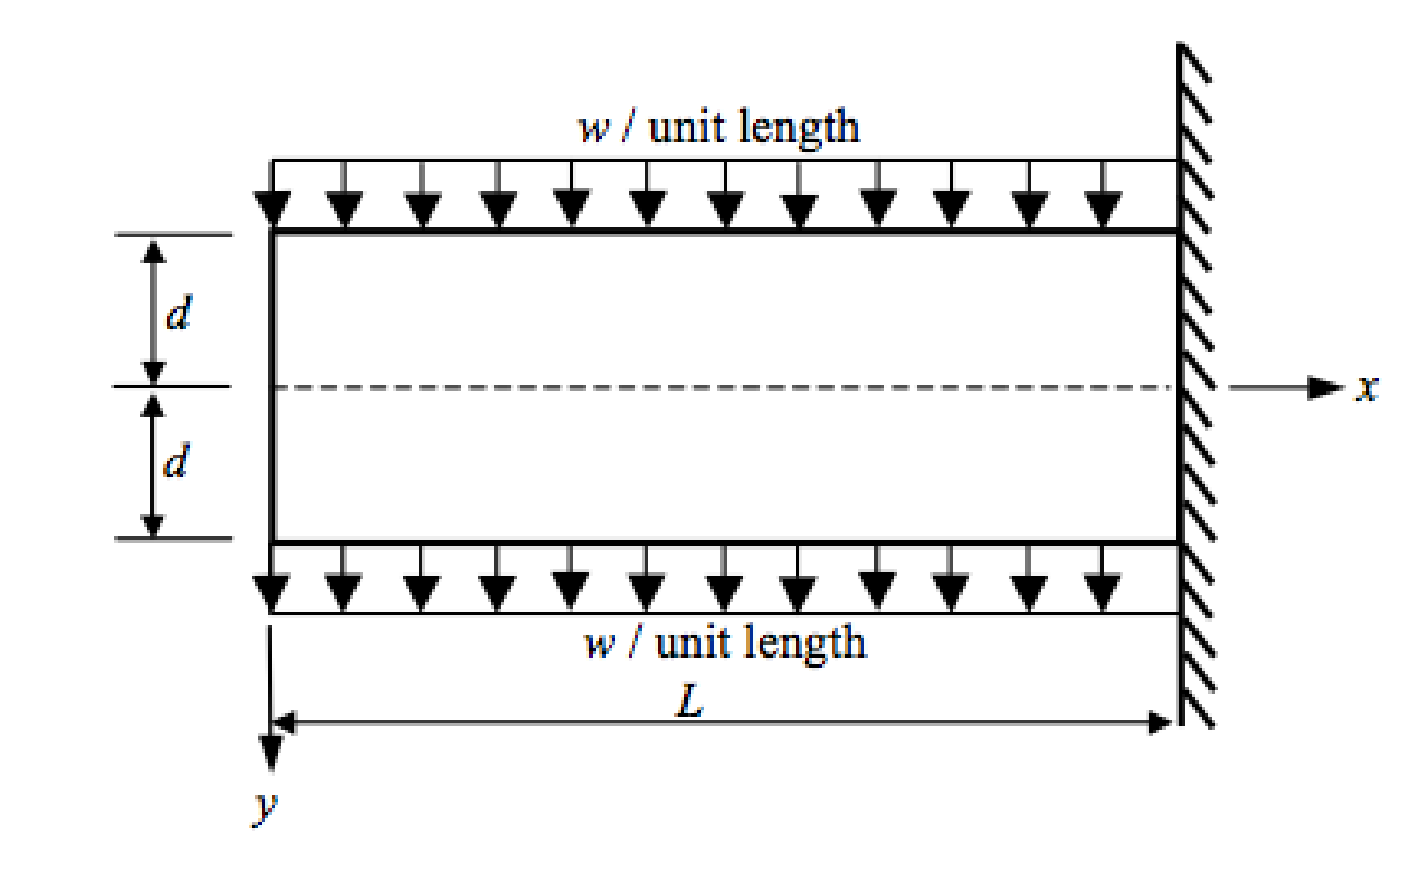
\includegraphics[width = 0.8\textwidth]{./img/diagram1.png}
    \caption{}
\end{figure}
Stress function:
\begin{equation}
    \phi = Ax^2 y + Bx^2 y^3 + Cy^5
\end{equation}
Check stress boundary conditions:
\begin{gather}
    \sigma_x = \frac{\partial^2 \phi}{\partial y^2} = 6Bx^2 y + 20Cy^3\\
    \sigma_y = \frac{\partial^2 \phi}{\partial x^2} = 2Ay + 2By^3\\
    \tau_{xy} = -\frac{\partial^2 \phi}{\partial x\partial y} = -2x\left(A + 3By^2\right)
\end{gather}
Check the boundary conditions. Lower surface:
\begin{gather}
    0 \leq x \leq L, \; y = d\\
    \left. \sigma_y \right|_{y=d} = 2Ad + 2Bd^3 \\
    \left. \tau_{xy} \right|_{y=d} = -2x(A+3Bd^2) = 0 \rightarrow A + 3Bd^2 = 0 \rightarrow A = -3Bd^2\\
    \therefore \left. \sigma_y \right|_{y=d} = -6Bd^3 + 2Bd^3 = w \rightarrow -4Bd^3 = w \rightarrow B = - \frac{w}{4d^3}\\
    \therefore A = \frac{3w}{4d}
\end{gather}
Upper surface (do not miss this step, make sure to check all boundaries):
\begin{gather}
    \left. \sigma_y\right|_{y=-d} = -2Ad -2Bd^3
\end{gather}
Substitute $A$ and $B$:
\begin{gather}
    \left. \sigma_y\right|_{y=-d} = -w\\
    \left. \tau_{xy} \right|_{y=-d} = 0
\end{gather}
Left surface:
\begin{gather}
    \left. \sigma_{x} \right|_{x=0} = 20Cy^3
\end{gather}
Resultant force:
\begin{gather}
    \int_{-d}^d \left(\sigma_x\right)\dif y = \int^d_{-d} \left(20Cy^3\right)\dif y = \left[5Cy^4\right]^d_{-d}= 0
\end{gather}
Resultant bending moment:
\begin{gather}
    \int_{-d}^d \left(\sigma_x \cdot y \right)\dif y =\int_{-d}^d \left(20Cy^4\right)\dif y = \left[4Cy^5\right]_{-d}^d = 8Cd^5 = 0\\
    \therefore C = 0
\end{gather}
Check Biharmonic relationship:
\begin{gather}
    \nabla^4 \phi = \frac{\partial^4 \phi}{\partial x^4} + 2\frac{\partial^4\phi}{\partial x^2 \partial y^2} + \frac{\partial^4 \phi}{\partial y^4} = 24By + 120Cy = 0\\
    C = -\frac{1}{5} B = \frac{w}{20d^3}
\end{gather}
We now have 2 values of $C$. Both are valid but we now can see that our stress function is wrong. $\phi$ is not a correct stress function! Refer to Question 2, to see the correct stress function. We do not have a $y^3$ term here.
\subsection{Question 7}
\begin{figure}[H]
    \centering
    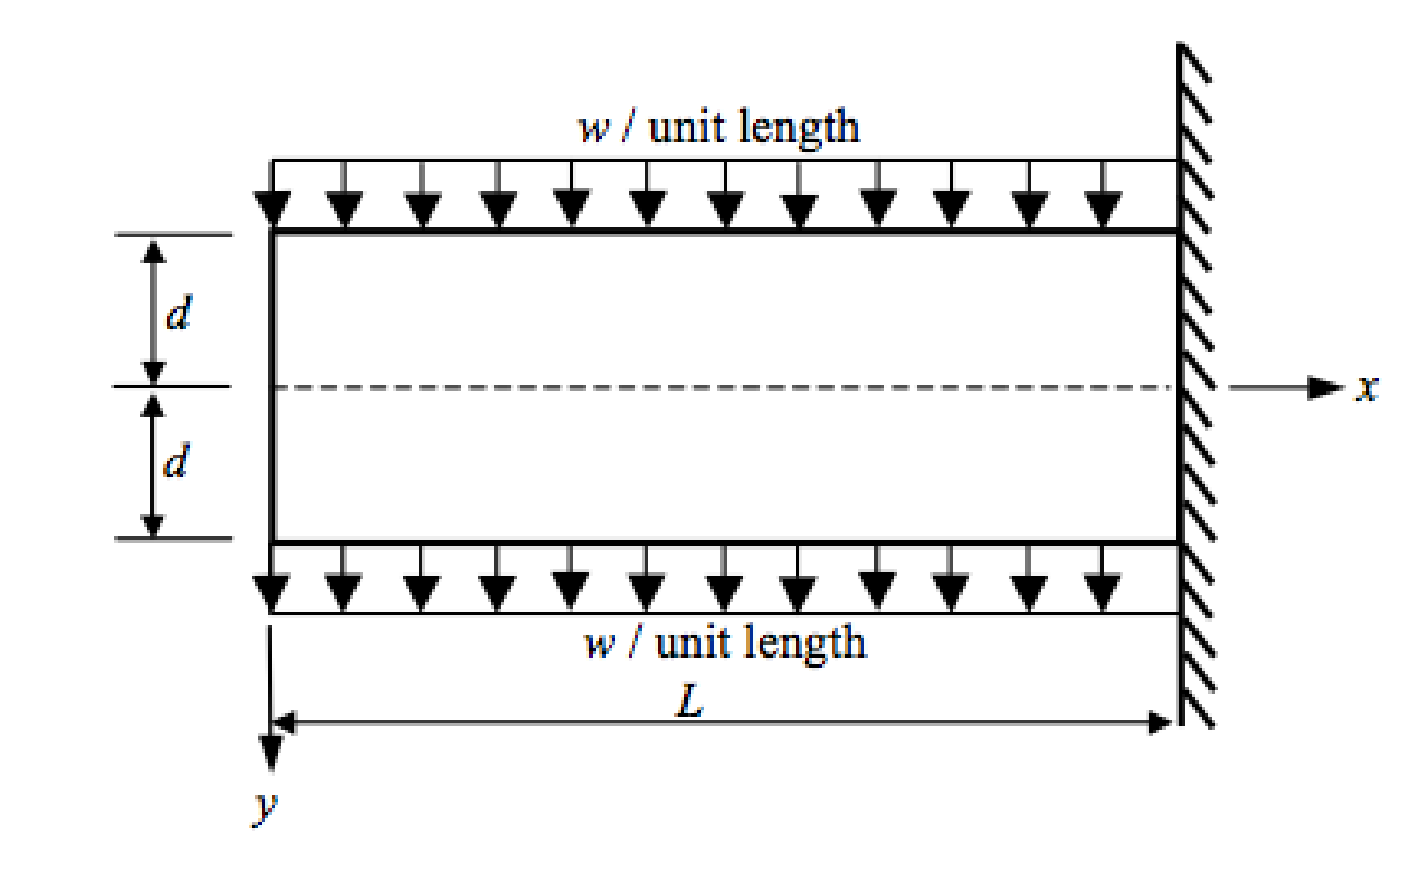
\includegraphics[width = 0.8\textwidth]{./img/diagram1.png}
    \caption{}
\end{figure}
Apply Biharmonic relationship:
\begin{gather}
    \phi_1 = \frac{wx^2}{8} \left[\left(\frac{y}{h}\right)^3-\frac{3y}{h} -2 \right] + Ay^3 - \frac{wy^5}{40h^3}\\
    \sigma_x = \frac{3w}{4}\frac{x^2y}{h^3} + 6Ay - \frac{w}{2}\frac{y^3}{h^3}\\
    \sigma_y = \frac{w}{4}\left(\frac{y^3}{h^3}-2-\frac{3y}{h}\right)\\
    \tau_{xy} = -\frac{3wx}{4}\left(\frac{y^2}{h^3} - \frac{1}{h}\right)
\end{gather}
Apply boundary condtions. Lower surface:
\begin{gather}
    \left. \sigma_y \right|_{y=-h} = \frac{w}{4}\left(-\frac{h^3}{h^3}-2 + \frac{3h}{h}\right) = 0\\
    \left. \tau_{xy}\right|_{y=-h} = -\frac{3wx}{4}\left(\frac{h^2}{h^3}-\frac{1}{h}\right) = 0
\end{gather}
Upper surface:
\begin{gather}
    \left. \sigma_y \right|_{y=h} = \frac{w}{4}\left(\frac{h^3}{h^3} - 2 - \frac{3h}{h}\right) = -w\\
    \left. \tau_{xy}\right|_{y=h} = 0
\end{gather}
Right side:
\begin{gather}
    \left. \sigma_x \right|_{x = L} = \frac{3w}{4}\frac{L^2y}{h^3} + 6Ay -\frac{w}{2}\frac{y^3}{h^3}
\end{gather}
Resultant force:
\begin{gather}
    \int_{-h}^h \left(\sigma_x\right)\dif y = \int_{-h}^h \left(\frac{3w}{4}\frac{L^2y}{h^3} + 6Ay -\frac{w}{2}\frac{y^3}{h^3}\right)\dif y = 0
\end{gather}
Resultant bending moment:
\begin{gather}
    \int_{-h}^h \left(\sigma_x \cdot y\right)\dif y = \int_{-h}^h \left(y\left(\frac{3w}{4}\frac{L^2y}{h^3} + 6Ay -\frac{w}{2}\frac{y^3}{h^3}\right)\right)\dif y = 0 \rightarrow A = ?
\end{gather}
Checking shear stress on right side:
\begin{gather}
    \left.\tau_{xy}\right|_{x=L} = -\frac{3wL}{4}\left(\frac{y^2}{h^3} - \frac{1}{h}\right)
\end{gather}
Resultant shear force:
\begin{gather}
    \int_{-h}^h \left(\tau_{xy}\right)\dif y = \int_{-h}^h \left(-\frac{3wL}{4}\left(\frac{y^2}{h^3}-\frac{1}{h}\right)\right)\dif y = wL
\end{gather}
Left:
\begin{gather}
    \left. \tau_{xy} \right|_{x = -L}\\
    \int_{-h}^h \left(\tau_{xy}\right)\dif y = - wL
\end{gather}
We can see that the shear stress on the left side is in the opposite direction to the external shear force, whereas on the left side it is in the same direction as the external shear force. We can see that we have a parabolic distribution of the shear stress, taking a maximum value of $\tau_{xy} = \frac{3wL}{4h}$.
\end{document}